\subsection{Streaming for End-Users}\label{sec:eup} % Martin

\begin{figure}[!h]
\centerline{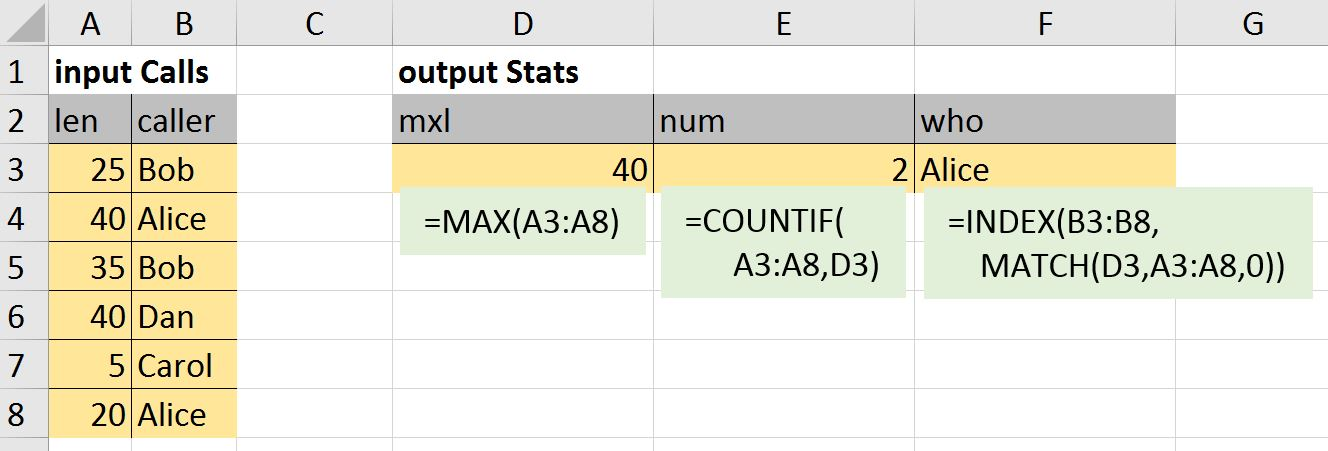
\includegraphics[width=\columnwidth]{CallStats.jpg}}
\vspace*{-4mm}
\caption{\label{fig:activesheets}ActiveSheets example.}
\end{figure}

We use the term \emph{end-users} to refer to users without particular
software development training. Probably the most successful
programming tool for end-users is spreadsheet formulas. And from the
early days of VisiCalc in 1979~\cite{bricklin_frankston_1979},
spreadsheet formulas have been \emph{reactive} in the sense that any
changes in their inputs trigger an automatic recomputation of their
outputs. Therefore, in 2014, Vaziri et al.\ designed \textsf{ActiveSheets}, a
spreadsheet-based stream programming model~\cite{vaziri_et_al_2014}.
Figure~\ref{fig:activesheets} gives an example that implements a
similar computation as Figure~\ref{fig:cql}.
Cells \lstinline{A3:B8} contain a sliding window of recent call
records, which ActiveSheets updates from live input data. Cells
\lstinline{D6:F6} contain the output data, \mbox{(re-)}com\-pu\-ted
using reactive spreadsheet formulas. The formula
\mbox{\lstinline{E6=COUNTIF(A3:A8,D6)}} counts how many calls in the
window are as long as a longest call. The formula
\mbox{\lstinline{F6=INDEX(B3:B8,F2)}} uses the relative index \lstinline{F2}
of the longest \lstinline{len} to retrieve the corresponding
caller.  ActiveSheets was influenced by
synchronous dataflow, discussed in Section~\ref{sec:sdf}.

After the initial ActiveSheets paper, there has been additional work
on using spreadsheets to develop stream processing applications.
ActiveSheets has been extended with time-based windows, key-based
partitions, and performance optimizations~\cite{hirzel_et_al_2016}.
And Chang and Myers hooked up streaming spreadsheets with REST APIs and
JSON~\cite{chang_myers_2015}.  Of course, spreadsheets are not the
only approach for end-user programming. For instance, META used a
controlled natural language for specifying event processing
rules~\cite{arnold_et_al_2016}. TEM used model-driven development
based on a spreadsheet~\cite{etzion_et_al_2016}. And MARIO even went
so far as to construct streaming applications automatically based on
search terms~\cite{riabov_et_al_2008}.
